\setchapterpreamble[u]{\margintoc}
\chapter{Sample and setup}
\labch{sample_and_setup}


\begin{quote}
\itshape

In this chapter we describe the setup and methods used in the experimental chapters. We describe the \Ca sample and the superconducting micro-resonator. We describe the assembly of the sample and its mounting in the dilution refrigerator along with the SMPD. Then, we present the resonator characterization at zero field and the protocol we use to tune the detection frequency of the SMPD to the resonator frequency. After this preliminary characterization, we summarize the magnetic-field alignment procedure and ensemble \Er spectroscopy using microwave photon counting. Finally, we outline the methods used to detect, address, and coherently control individual \Er spins, as well as characterize their relaxation and decoherence times.

\end{quote}

\section{Sample}
\labsec{sample_details}

The experiments reported in this thesis were all carried out on one monocrystalline \Ca sample on the surface of which a superconducting thin-film resonator was fabricated. 

The sample originates from a large single-crystal \textit{boule} grown by Philippe Goldner using the Czochralski~\sidecite{erb_growth_2013} method from CaCO3 (99.95\% purity) and WO3 (99.9\% purity). No paramagnetic impurities were added during crystal growth. Standard EPR measurements performed by Sylvain Bertrana on a sample from the same \textit{boule} yield a residual \Er concentration of 3.1(2)~ppb~\sidecite{ledantec_electron_2022}. The average distance between \Er ions at this concentration is 300~nm, far enough to suppress dipolar interactions between the \Er spins.

The sample used in this work was cut into a rectangular slab. Its dimensions are 7 mm by 4 mm by 2 mm, with its surface approximately along the $(a,c)$-plane of the crystal and the $c$-axis along the short edge. The polishing of the surface, performed by SurfaceNet GmbH, reduced the thickness to 0.5~mm.

% The nuclear-spin environment of \Ca is dominated by \W nuclear-spins, which have a natural abundance of 14.4\% and a remarkably low gyromagnetic ratio $\gamma_{\text{\W}}/2\pi = 1.77394$~MHz/T \sidecite{knight_solidstate_1986}. The combination of a low density of nuclear-spins and a weak gyromagnetic ratio results in an environment with a reduced magnetic moment density. As such, the magnetic noise perceived by any paramagnetic impurity hosted in the crystal is significantly smaller when compared to other hosts used in quantum applications, such as yttrium orthosilicate (Y$_2$SiO$_5$) and yttrium oxide (Y$_2$O$_3$). Extremely low doping and low magnetic moment density are crucial for achieving long spin coherence, as demonstrated by previous work of the group performed by Marianne le Dantec, where ensemble coherence times up to 23~ms were measured in a sample of similar characteristics \sidecite{ledantec_twentythreemillisecond_2021}. 

\subsection{Resonator design and fabrication}

As discussed in \refch{spins_coupled_to_a_cavity}, the purpose of the resonator is to enhance the radiative relaxation of the spins via the Purcell effect. To achieve this, the coupling strength $g_0$ must be maximized. From Eq.~\ref{eq:coupling_strength_nanowire}, we observe that the coupling strength scales inversely with the resonator impedance. Consequently, reducing the resonator impedance provides a direct route to increasing the coupling rate. We achieve this through a design that maximizes the resonator capacitance while keeping the resonator inductance to a minimum. 

The resonator is made of a 50-nm-thick niobium film and takes the form of two superconducting electrodes separated by an interdigitated capacitor and shunted by a small constriction: a nanowire with a length of 50~\textmu m and a width of 300~nm parallel to the $c$-axis. A micrograph of one of the resonators is shown in \reffig{sample}a. Each of the fingers has an associated geometric inductance as the current needs to travel from one side of the capacitor plate to the other. The geometric inductance increases the impedance of the resonator without contributing to the magnetic field generated by the nanowire and is therefore important to minimize. To reduce the effect of the finger's geometric inductance the "bow tie" design shown in the micrograph was adopted.

We use finite element simulations using \texttt{HFSS} to target the frequency and impedance of the resonators. The simulations follow the procedure developed by Zhiren Wang and Marianne le Dantec, which is described in detail in refs.~\sidecite{ledantec_electron_2022, wang_addressing_2023}. The key modification implemented in this work was the reduction of the nanowire width from 500~nm to 300~nm, resulting in an increased magnetic coupling strength to the \Er spins.

We measure the impedance of the resonator by introducing a small lumped element with inductance $\delta L$. We run the simulation for different values of inductance and obtain the frequency as a function of $\delta L$, which is then fit to $1/\sqrt{(L+\delta L)\,C}$~\sidecite{eichler_electron_2017}. From the values of $L$ and $C$ we obtain $Z_r=13$~$\Omega$. 

The simulations also yield the current density through the nanowire, which was used by André Pscherer to create a spin coupling map based on the magnetic field generated by the rectangular nanowire using COMSOL (see \reffig{sample}b). For an \Er spin located 10--100~nm away, we expect $g_0/2\pi = 8$--$12$~kHz, about twice as large as in the previous design (see Figure 3.4b in ref.~\cite{wang_addressing_2023}).

\begin{figure*}
    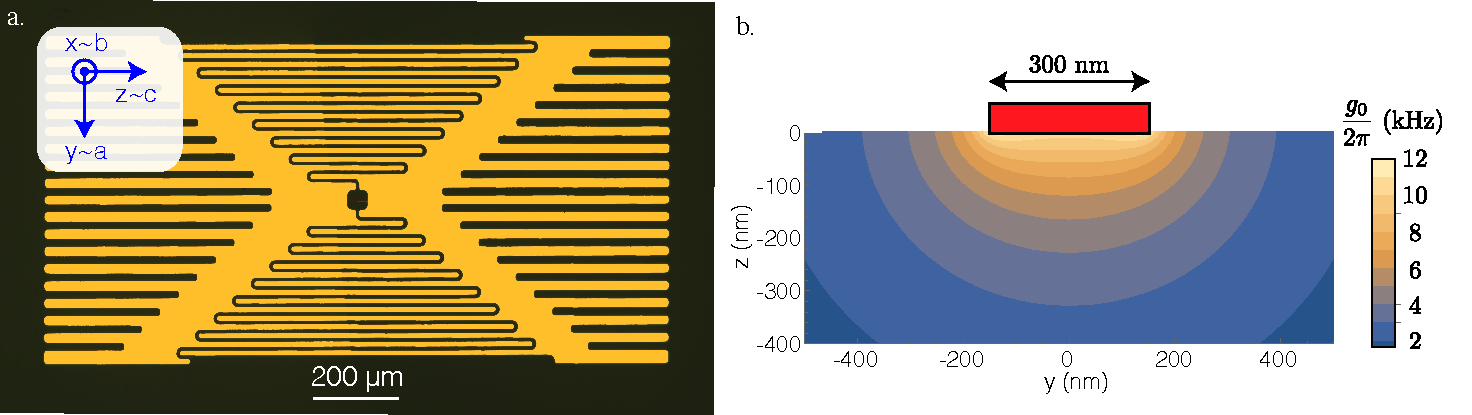
\includegraphics{chapter2/figures/sample.pdf}
    \caption[Sample micrograph and coupling map]{Sample micrograph and coupling map. \textbf{a.} False color micrograph of a Nb thin-film resonator of the same design fabricated on a \Ca crystal. The nanowire is colored in red while the rest of the resonator is colored yellow. The picture is stitched from 2 independent images. The laboratory frame axes $x$, $y$ and $z$ approximately coincide with the crystal axes. The $z$-axis is parallel to the nanowire and the $x$-axis is perpendicular to the plane. 
    \textbf{b.} Spatial map for the coupling $g_0$ between \Er and the superconducting resonator calculated with COMSOL by André Pscherer. The map is shown as a transversal cut around the nanowire (in red).}
    \labfig{sample}
\end{figure*}

Three superconducting resonators of similar design are fabricated on top of the \Ca sample. The target frequencies of the resonators are separated by $50$~MHz, to increase the probability that at least one of them lies within the SMPD range. The fabrication also follows the process developed by Zhiren Wang and Marianne le Dantec, which is outlined in the following.

\begin{itemize}
    \item Surface cleaning with a mixture of sulfuric acid and hydrogen peroxide.
    \item Sputtering of a 50~nm thick Nb film.
    \item A double layer of PMMA and MMA positive resist is spin coated on top of the chip. The respective thicknesses are 340~nm and 110~nm.
    \item A single electron beam lithography step patterns the resonator on the sample. The exposed resist is subsequently removed.
    \item A 30~nm film of aluminum is evaporated on the sample to act as a hard mask. 
    \item Aluminum lift-off.
    \item Reactive ion etching removes the unmasked Nb film.
    \item Aluminum removal through wet-etching.
\end{itemize}

When characterizing the resonators we found that their frequencies were $\sim100$~MHz higher than the target ones and therefore outside the SMPD range. We reworked the resonators by removing Nb from the fingers, therefore increasing the distance between the capacitors and reducing their frequency. The rework had to be performed twice. During one of these reworks, the sample was snapped into two halves, leaving one resonator unharmed, which was then found to have the appropriate frequency. We qualitatively note that the quality factor of the resonator was significantly reduced after the rework.

\subsubsection{Sample assembly}

\begin{figure*}
    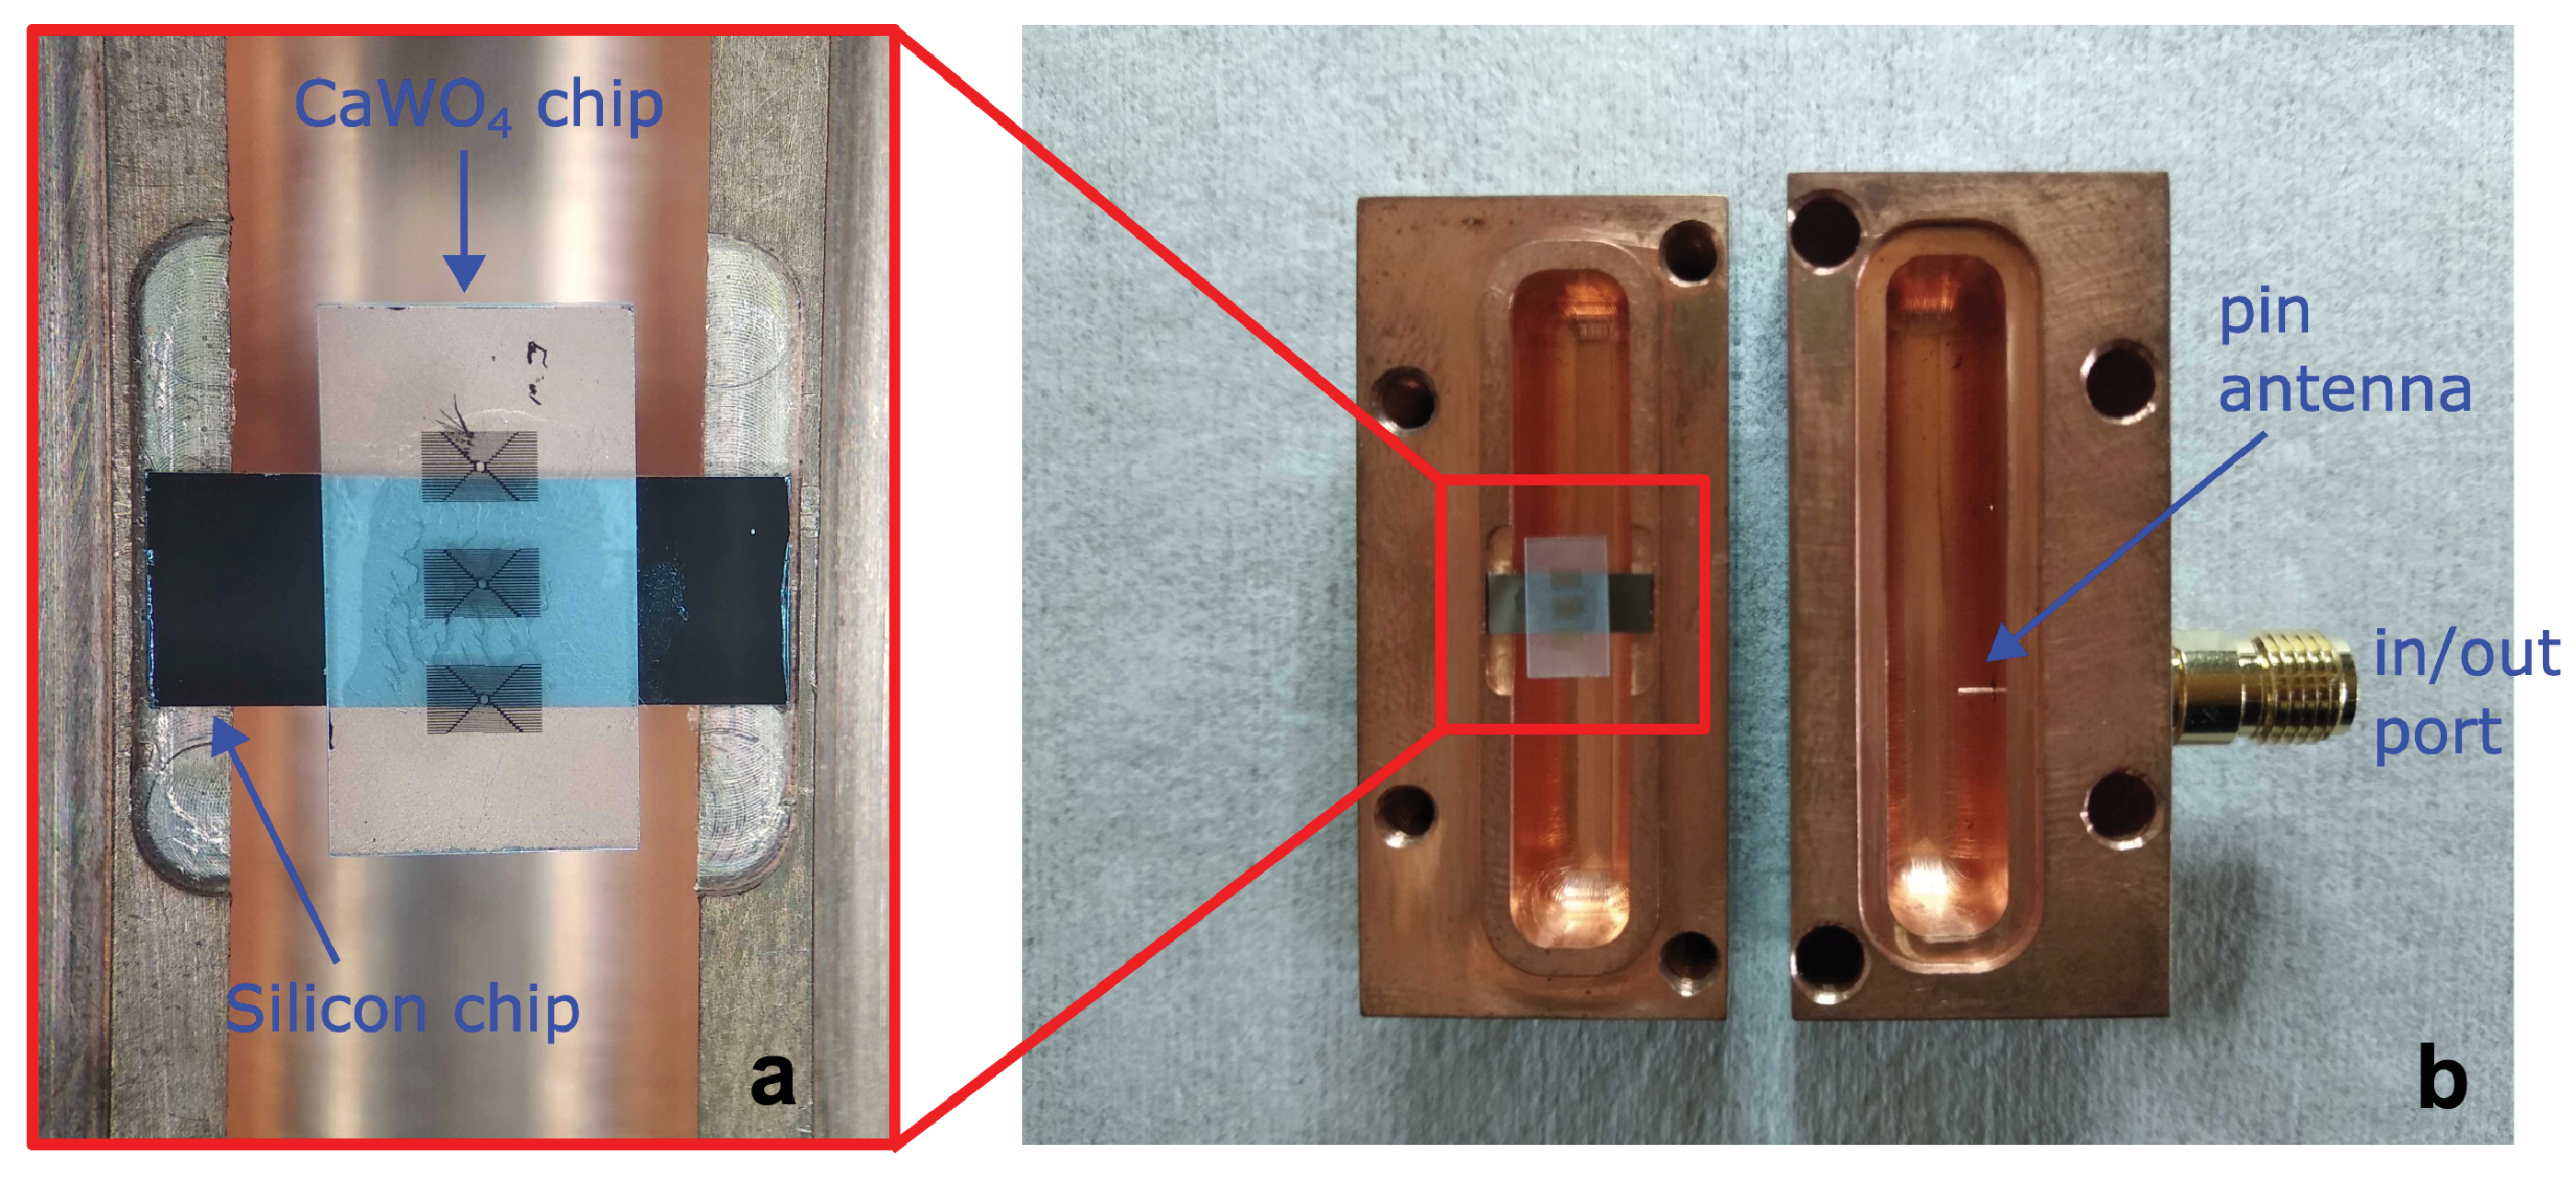
\includegraphics{chapter2/figures/resonator_assembly.pdf}
    \caption[Resonator assembly]{Resonator and copper cavity assembly. Since the sample remains in the fridge at the time of writing this manuscript, the image was taken from ref.~\cite{wang_addressing_2023}, which used a similar assembly.
    \textbf{a.} Zoomed view of the sample. The \Ca sample in the figure is $4 \times 7$~mm and three resonators have been fabricated on top. We note that in the real sample used for this work, the chip broke during fabrication but left one resonator unharmed. The sample is affixed to a silicon bridge (dark rectangle) supported by the copper cavity.
    \textbf{b.} Open copper cavity. The cavity is set up in the reflection configuration, where only one metallic antenna is present. The antenna is soldered to a SMA port which connects to the microwave lines. A second hole (visible as a small speck on top of the antenna) is used to introduce a second antenna in the transmission configuration. The hole is covered with copper tape on the outside in the reflection setup.}
    \labfig{resonator_assembly}
\end{figure*}

The sample is mounted in a copper sample holder as shown in \reffig{resonator_assembly}. The sample is affixed with vacuum grease to a silicon chip that plays the role of a bridge by suspending it in the center of the cavity. The silicon chip is held in place by compression between the cavity halves. The resonator is capacitively coupled to an antenna that is soldered to an SMA connector. The antenna protrudes through a small pinhole in the cavity wall, and coupling to the resonator is tuned by adjusting the insertion depth. The copper cavity is then mounted on the fridge with a three-axis magnet surrounding the assembly. 

During this work, two different setups were used: first, in Chapters \ref{ch:detection_and_control_of_individual_w} \& \ref{ch:individual_nuclear_spins_quantum_information} we use a reflection configuration with a single pin antenna. The coupling of the antenna to the resonator is tuned to achieve critical coupling. Second, in Chapter \ref{ch:nb_nuclear_spin} a transmission setup is used, where the resonator is coupled with two antennas to separate lines, one for input and one for output. The coupling rates of the two antennas are dissimilar by a factor $\sim10$, with the larger one being the output line, so that most of the fluorescent photons are directed towards the detector. 

\begin{figure*}[t!]
    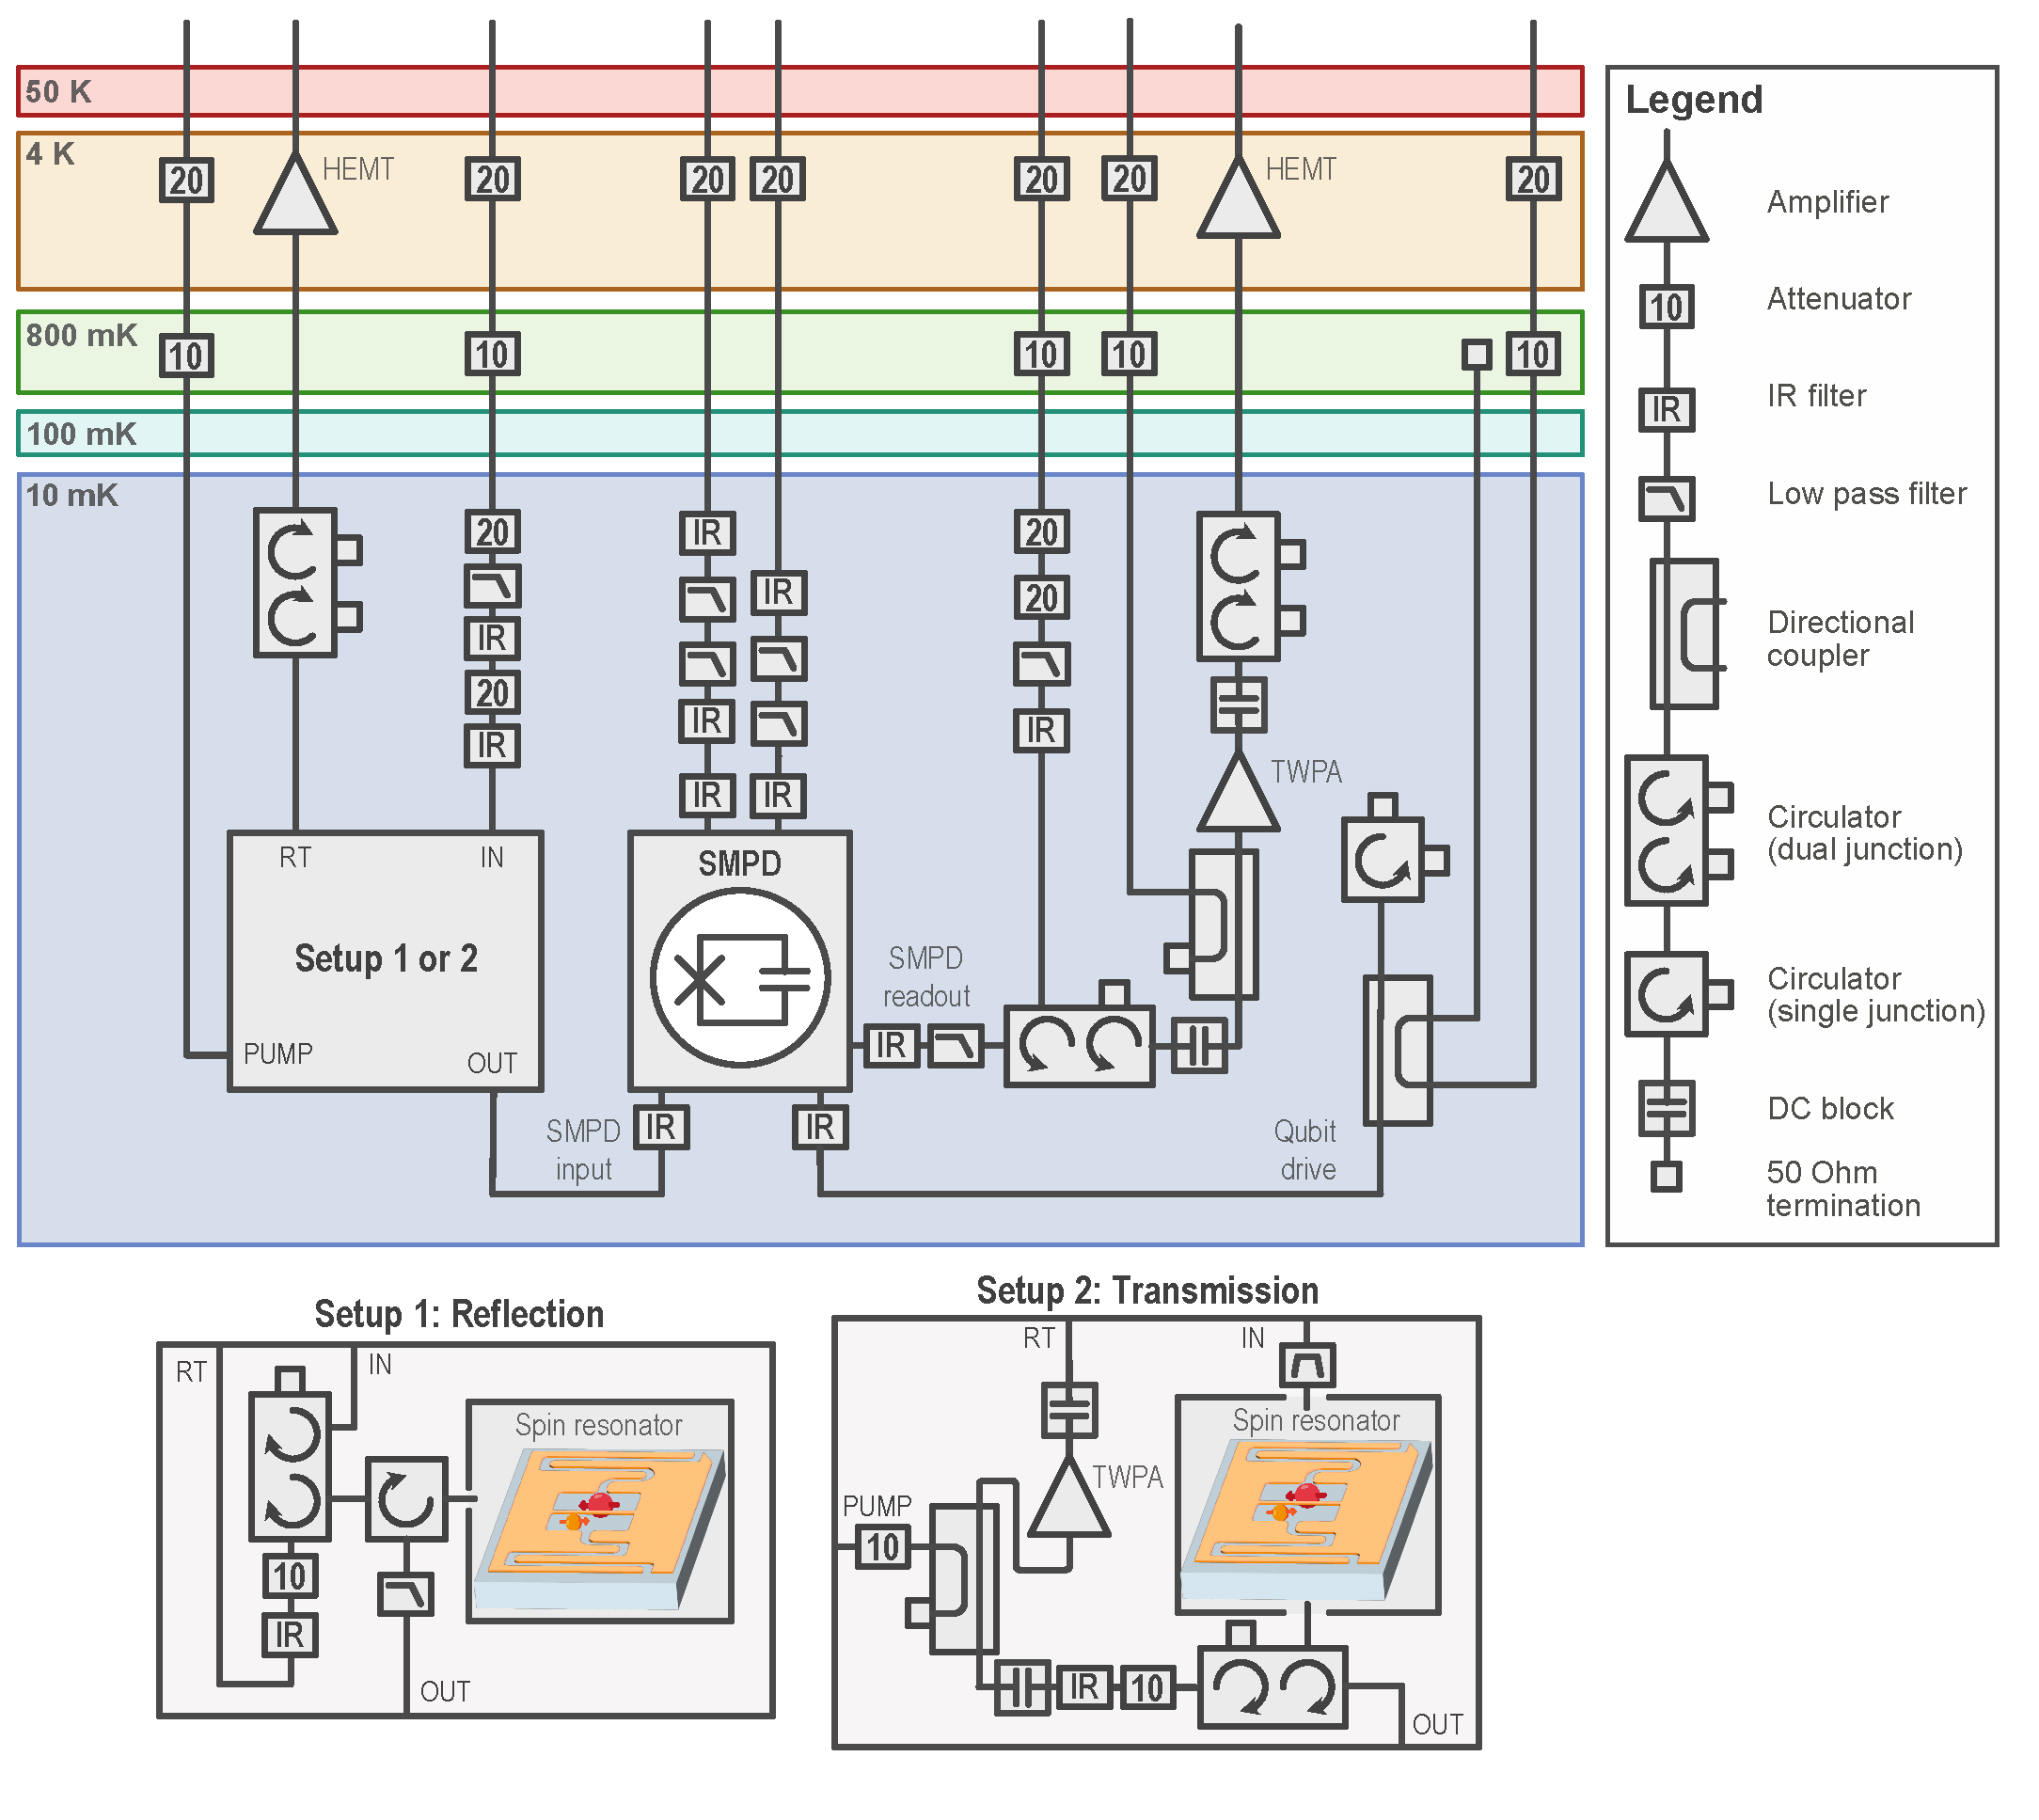
\includegraphics{chapter2/figures/wiring_diagram.pdf}
    \caption[Wiring diagram]{Cryogenic wiring diagram with the two configurations used in this work. Two different setups were used during the course of this thesis. The main changes are outlined in the bottom separating the components between the reflection and the transmission setups. Line names are marked at the top which indicate: $i$ for input, $o$ for output, $p$ for TWPA pumping and $dc$ for DC bias lines. For the transmission setup, a large \textmu-metal shield surrounding the dilution fridge at room temperature was introduced to shield the interior from stray magnetic fields.}
    \labfig{wiring_diagram}
\end{figure*}

\section{Measurement setup}
\labsec{measurement_setup}

Both the sample and the SMPD are mounted at the $10$~mK stage of a dilution refrigerator. The wiring diagram of the fridge is presented in \reffig{wiring_diagram}. Line $i1$ is directly connected to the SMPD input and is therefore well attenuated (-20 dB at 4~K, -10 dB at 800~mK, -40 dB at 10~mK) to reduce the number of thermal photons per mode. Reducing the thermal population at the input of the detector is required to achieve low dark counts and high SNR, as discussed in Appendix \ref{app:SMPD}.

%We use microwave coaxial cable and low temperature components to deliver the microwave signals. The experiments need to be carried at low temperatures, since the SNR of the SMPD is closely tied to the thermal population of the environment. Reducing the temperature will exponentially suppress microwave thermal radiation at the input as the qubit population, enhancing the SNR of the detector\sidenote{For a more comprehensive study of the detector SNR and, we direct the reader to the thesis of Louis Pallegoix~\cite{pallegoix_high_2025}, who fabricated and characterized the device used during these experiments.}. In addition, we use a superconducting microwave cable to minimize the losses between the resonator and the SMPD.

Two configurations were used to measure the sample: in reflection (Chapters \ref{ch:detection_and_control_of_individual_w} \& \ref{ch:individual_nuclear_spins_quantum_information}), and in transmission (Chapter \ref{ch:nb_nuclear_spin}). For the transmission setup, a large \textmu-metal shield surrounding the dilution fridge at room temperature was installed to shield the interior from stray magnetic fields.

%As with the cavity setup, we note that two measurement configurations were employed: a reflection and a transmission configuration (see \reffig{wiring_diagram}). These correspond to the two experimental runs that comprise the bulk of the results\sidenote{The motivation for switching to the transmission configuration was the expectation that placing the microwave cavity between the room-temperature environment and the SMPD input would reduce the flux of thermal photons reaching the detector and therefore lower the dark-count rate. In practice, we did not measure any significant effect.}. In addition, in the transmission setup a 

The sample is surrounded by a 1T/1T/1T superconducting vector magnet, which can produce an arbitrary vector field along the three orthogonal directions $X$, $Y$ and $Z$. The coils are independently driven by three current sources which can be individually shunted on demand with superconducting wires, turning on the so-called magnet persistent mode in which field stability is greatly enhanced. All measurements reported in the experimental chapters on individual spins were taken in this persistent mode. %Given that the resonator is a superconducting film, the magnetic field needs to be applied on the plane of the resonator, as small out-of-plane component will strongly reduce its quality factor.

The SMPD (described in \refsec{Detecting_individual_Er}) is placed inside a light-tight container with a \textmu-metal shield to protect the device from stray magnetic fields. The SMPD pump is sent through line $i3$. The frequency and bandwidth are tuned by sending current through lines $dc1$ and $dc2$, respectively. 
In the reflection setup, we use $i1$ to tune the SMPD parameters (pump frequency and amplitude) to achieve maximum detection efficiency. In the transmission setup, the SMPD input line is filtered by the resonator. We instead use the qubit drive line ($i3$), which is weakly capacitively coupled to the buffer for characterization. Qubit readout pulses are sent through line $i2$, and the reflected signals are directed to output line $o1$, which contains a Traveling Wave Parametric Amplifier (TWPA) pumped through line $p1$.

\section{Superconducting resonator characterization}

The resonator is first characterized at zero magnetic field using a Vector Network Analyzer in the reflection configuration. \reffig{resonator_fit}a shows the complex reflection parameter as a function of frequency. By fitting the model, we obtain the internal and coupling losses of the resonator, $\kappa_i/2\pi=255$~kHz and $\kappa_c/2\pi = 621$~kHz. The quality factor of the resonator is given by 

\begin{equation}
    Q = \frac{\omega_r}{\kappa_i + \kappa_c} = 8.8 \times 10^{5}
\end{equation}

\begin{marginfigure}
    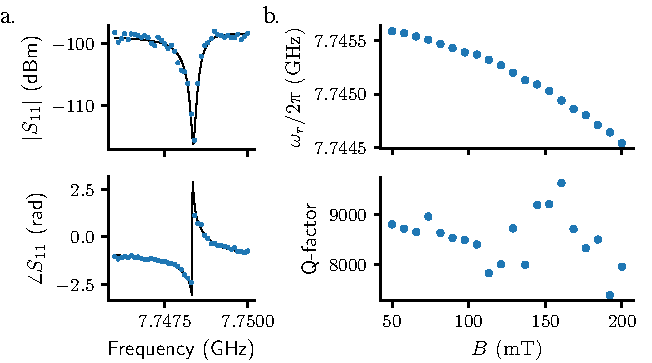
\includegraphics{chapter2/figures/resonator_fit.pdf}
    \caption[Resonator fit]{Resonator fit at zero field. 
    Reflection signal of the resonator at zero magnetic field. The data is fit to a standard reflection model (black lines) which yields $\omega_r/2\pi=7.74845$~GHz and a quality factor of $Q=8.8\times10^5$.
    }
    \labfig{resonator_fit}
\end{marginfigure}

\subsection{Magnetic field alignment}

During the mounting process, the resonator assembly is fixed such that the $Y$ and $Z$ axes of the magnet are close to the plane of the resonator. Due to the limited precision of manual alignment, we begin the experimental run by measuring the relative alignment between these coordinate frames. We follow the procedure described in ref.~\sidecite{dantec_electron_2022}, which we briefly summarize below.

\begin{figure}
    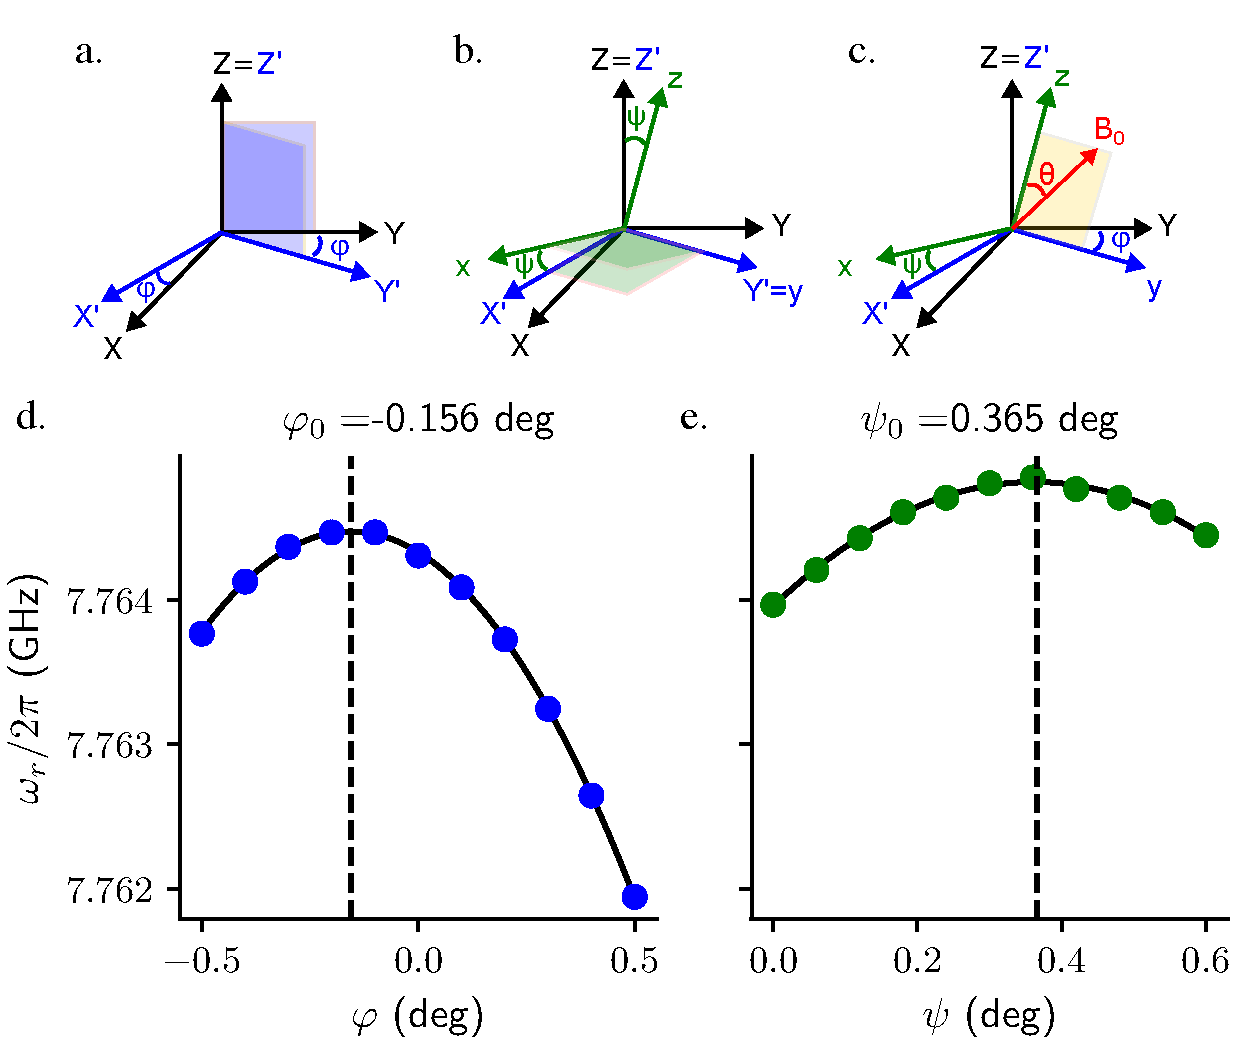
\includegraphics{chapter2/figures/b_field_alignment_scheme.pdf}
    \caption[Magnetic field alignment]{Magnetic field alignment scheme and data. Figures a, b and c show the subsequent rotations performed to arrive to the resonator reference frame. Figures d and e plot the frequency of the resonator as a function of the out-of-plane angle during steps 2 and 5 of the aligning procedure (see text). The data were fit to a parabola and the alignment angles $\varphi_0$ and $\psi_0$ correspond to the top of the parabolic fit.}
    \labfig{field_alignment}
\end{figure}

The working principle of the alignment procedure is the strong dependence of the resonator frequency on any out-of-plane component of the magnetic field \sidenote{A magnetic field increases the penetration depth, and therefore the kinetic inductance. This results in a reduction of the resonator frequency. This effect is also present for in-plane fields but is drastically stronger for out-of-plane components.}. By measuring the dependence of the frequency on the components of the field we can map a rotation from the magnetic-field axes $X$, $Y$, and $Z$ to the resonator-plane axes $x$, $y$, and $z$ (see \reffig{sample}). The steps of the procedure, shown in a diagram in \reffig{field_alignment}, are:

\begin{enumerate}
    \item Apply a 50~mT field along the $Y$ axis.
    \item Sweep the amplitude of a small magnetic field along the $X$ axis and measure the frequency of the resonator. The combined field makes an angle $\varphi$ with respect to the $(Y, Z)$-plane. We measure the angle for which the resonator frequency is maximized, $\varphi_0$, which defines the intermediate coordinate frame $X'$, $Y'$, and $Z$ (see \reffig{field_alignment}a). 
    \item Ramp down the magnetic field along $Y$ to 0~mT.
    \item Ramp up the magnetic field along $Z$ to 50~mT.
    \item Repeat the procedure described in step 2. The angle $\psi_0$ in the ($Y'$, $Z$)-plane defines the aligned coordinate system $x$, $y$, and $z$ (see \reffig{field_alignment}b). 
    \item Define $\theta$ as the angle in the resonator plane with respect to the $z$ axis (see \reffig{field_alignment}c).
\end{enumerate}


The resonator frequency as a function of $\varphi$ and $\psi$ is plotted in \reffig{field_alignment}d and \reffig{field_alignment}e, respectively. The data were fit to a parabola and the top gives the values of $\varphi_0$ and $\psi_0$. The applied magnetic field in the resonator plane can then be expressed in the laboratory frame as

\begin{equation}
    \mathbf{B}_{0} = B_{0}
    \begin{pmatrix}
    \sin \theta \, \sin \phi_0 - \cos \theta \, \sin \psi_0 \, \cos \phi_0 \\
    \sin \theta \, \cos \phi_0 + \cos \theta \, \sin \psi_0 \, \sin \phi_0 \\
    \cos \theta \, \cos \psi_0
    \end{pmatrix}
\end{equation}

In the following, the magnetic field will always be applied in the plane of the resonator, unless otherwise stated.

\begin{figure}
    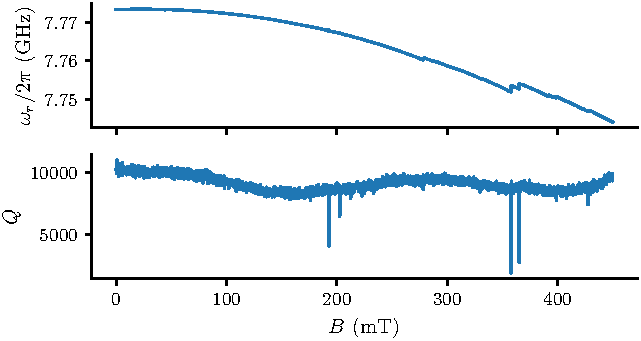
\includegraphics{chapter2/figures/resonator_vs_bfield.pdf}
    \caption[Resonator response to in-plane field]{Resonator response to in-plane magnetic field. Frequency and quality factor as a function of in-plane magnetic field amplitude. The data was taken in transmission mode.}
    \labfig{resonator_vs_bfield}
\end{figure}

We then measure the frequency and quality factor as a function of the applied field. The data are shown in \reffig{resonator_vs_bfield}. The resonance frequency is quadratically shifted as a function of the in-plane field. At 450~mT it drops approximately 40~MHz with respect to the zero field values. Due to the field alignment, the quality factor of the resonator remains approximately constant as a function of the magnetic field. We note that the sharp peaks correspond to paramagnetic impurities previously observed in similar samples~\sidecite{ledantec_electron_2022,billaud_electron_2025}.

%We then measure the resonance frequency $\omega_{r}$ and the internal losses $\kappa_{i}$ of the superconducting resonator show a response to the externally applied magnetic field. 

%These shifts are due to the niobium film kinetic inductance dependence on the magnetic field. The magnitude and character of this response depend on the alignment of the $B_0$ relative to the plane of the superconducting resonator film. 

%In contrast, the resonator response to an out-of-plane field component is considerably more dramatic, even a marginal perpendicular component of $B_{0}$ can lead to significant inductive shifts and enhanced dissipative losses. 

\section{SMPD frequency tuning}

%We now describe the frequency calibration procedure of the SMPD used to tune the input frequency of the detector to the spin resonator. This procedure is required both as an initial calibration as well as measurements where the magnetic field is swept as the frequency of the resonator will shift with the applied field (see \reffig{resonator_fit}b). 

The first step of the measurements is to tune the SMPD frequency to the resonator frequency $\omega_r$. The procedure is fully automated, as explained below. This is needed in particular when large magnetic field sweeps are launched, since $\omega_r$ then changes with field, thus necessitating repeated SMPD tuning during the sweep. %The procedure is typically repeated every 1~mT.

To achieve this, we sweep a weak probe tone around the resonator frequency on $i1$ while varying the voltage applied to the DC tuning line $dc1$ to tune the input frequency of the detector. In the reflection measurement, the signal reflected on the resonator reaches the SMPD input. In the transmission measurement, the probe tone is filtered by the resonator before reaching the SMPD input.

\begin{figure}
    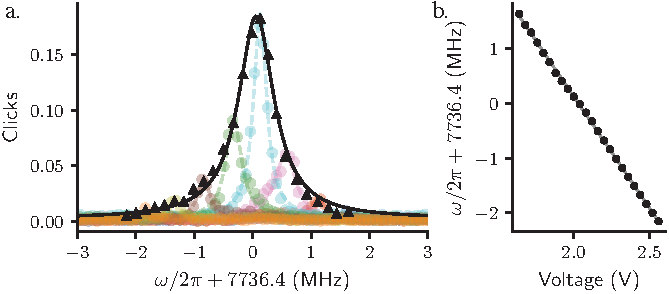
\includegraphics{chapter2/figures/buffer_autocalibration.pdf}
    \caption[Buffer frequency tuning]{SMPD buffer resonator frequency calibration in transmission configuration.
    \textbf{a.} Response of the SMPD as a function of probe frequency for different DC tuning voltages (faintly colored circles). For clarity only a few have been plotted. Each trace is fitted to a Lorentzian (faint dashed lines), yielding narrow linewidths of approximately 300 kHz. The extracted peak centers (black triangles) form an envelope reflecting the resonator response. Fitting the envelope to a Fano resonance yields a resonator linewidth of 740 kHz.
    \textbf{b.} SMPD resonance frequency as a function of DC bias voltage, showing a linear dependence used to tune the SMPD to the resonator frequency.}
    \labfig{buffer_autocalibration}
\end{figure}



We now show an example of frequency tuning, performed with the transmission setup. \reffig{buffer_autocalibration}a shows the SMPD response for different DC voltages which appears as a set of narrow resonance lines with linewidths of approximately 300 kHz (the SMPD bandwidth). Each individual trace is well described by a Lorentzian lineshape, and the extracted peak positions (red triangles) form a broader envelope corresponding to the resonator response. Fitting this envelope yields a resonator linewidth of 740 kHz. We observe a slight asymmetry in the envelope lineshape, which we attribute to weak parasitic transmission between the two antennas interfering with the resonant response. This asymmetry is well captured by a Fano model; however, the extracted linewidth agrees with the Lorentzian fit within uncertainty, and the large Fano asymmetry parameter indicates that the parasitic contribution is weak and does not affect the linewidth determination. %In contrast, for the reflection measurement the resonator appears as a dip on the detected amplitude, and a resonator model is enough to capture the behavior as there is no parasitic transmission.

In \reffig{buffer_autocalibration}b, the SMPD resonance frequency is plotted as a function of the applied DC voltage and fitted with a linear relation. Using this calibration, we set the DC voltage corresponding to the resonator frequency, thereby aligning the SMPD to the resonator. 
%This information is also used to tune the SMPD frequency across different electron transition frequencies in Fig. \ref{fig1}c since they span wider than the SMPD bandwidth.

\section{Erbium ensemble spectroscopy}
\labsec{erbium_spin_detection}

We now perform spectroscopy of the \Er spin ensemble. Given the gyromagnetic ratio of \Er spins (see \refsec{erbium_ions_in_ca}), the expected magnetic field along the $c$-axis for which the resonator is tuned to the ensemble is given by

\begin{equation}
    B_0 = \frac{\omega_r}{\gamma_\parallel} \approx 440~\text{mT} 
\end{equation}

We ramp the magnetic field along the $z$-axis (which is close to the $c$-axis) to this value and perform photon counting spectroscopy. We apply a strong microwave pulse with a duration of 100~\textmu s at the frequency of the resonator $\omega_r$. After the pulse, we measure the number of counts on the SMPD during an integration window of $\tau_\text{int}=200$~ms. We average the total number of counts during the integration time over a number of iterations to obtain the ensemble average counts $\langle C \rangle$. We repeat this measurement while sweeping the magnetic field. Due to the dependence of the resonator frequency on the applied magnetic field, we apply the SMPD frequency tuning procedure for every value of $B_0$ ($0.15$~mT steps). 


\begin{figure}
    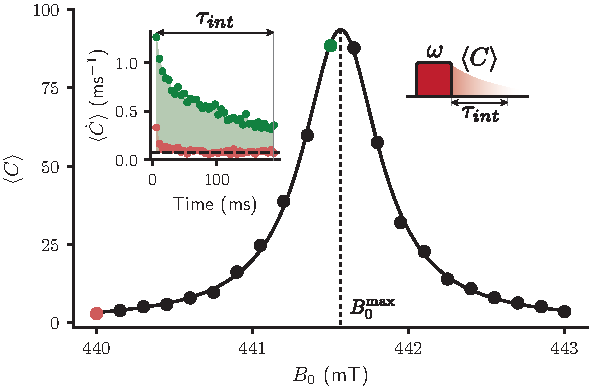
\includegraphics{chapter2/figures/high_power_spectroscopy.pdf}
    \caption[High power spectroscopy]{High power spectroscopy. Ensemble average of counts after microwave excitation $\langle C \rangle$ as a function of the magnetic field along the $z$-axis. The data points are fit to a Lorentzian curve (black line) centered at $B_0^\mathrm{max}$. \textit{Top right inset.} Pulse sequence. \textit{Top left inset.} Microwave count rate as a function of time for the green and red data points. The integral of the curve, which corresponds to $\langle C \rangle$, is highlighted with the respective colors. The dark count rate of the SMPD is plotted as a dashed horizontal line.}
    \labfig{high_power_spectroscopy}
\end{figure}


\reffig{high_power_spectroscopy} shows $\langle C \rangle$ as a function of $B_0$. We observe a peak at $B_0^\text{max}=441.5$~mT of width $0.6$~mT, which corresponds to the resonance of \Er spins. The inset plot shows the count rate $\langle \dot C \rangle$ after the excitation pulse at $t=0$ for two different magnetic fields (marked as red and green markers in the main figure). When the resonator is not resonant with the ensemble (red curve), the count rate is flat and equal to the dark count rate of the SMPD, shown as a black dashed line. The first point of the curve escapes that trend, and we attribute this increase in counts to the emission of unknown degrees of freedom in the resonator, such as TLS~\sidecite{wang_addressing_2023}. In contrast, when the ensemble is resonant the count rate displays a non-exponential decay over a period of time longer than 200~ms. This non-exponential behavior is consistent with the excitation of an ensemble of \Er spins with different coupling strength, and therefore relaxation rate. This phenomenon is quantitatively described in ref.~\sidecite{billaud_electron_2025}.

Due to finite precision when cutting the sample, the crystal $c$-axis is not perfectly parallel to the surface plane (which corresponds to the $(y, z)$-plane). We define $\theta$ as the angle of $B_0$ with respect to the projection of the $c$-axis on the $(y, z)$-plane. In addition, we define $\beta$ as the angle made by $B_0$ with the $(y, z)$-plane. Finally, we define $\beta_0$ as the angle between the $c$-axis and the $z$-axis (see \reffig{sample_field_alignment} inset).

\begin{figure}
    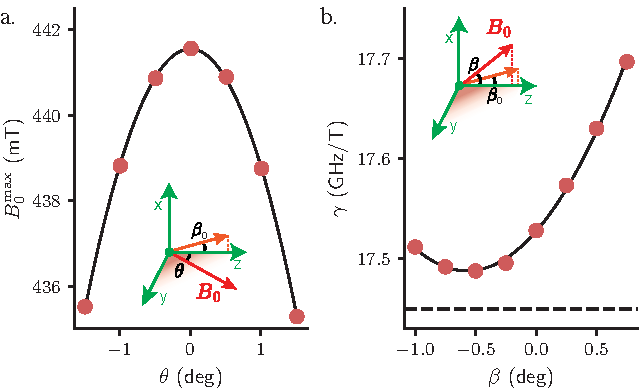
\includegraphics{chapter2/figures/sample_field_alignment.pdf}
    \caption[Sample Field Alignment]{Sample Field Alignment. 
    \textbf{a.} \Er main line resonant field as a function of the in-plane angle $\theta$. The data is fit to a parabola (black line).
    \textbf{b.} Gyromagnetic factor $\gamma$ as a function of the out-of-plane angle $\beta$ for $\theta=0$. The parabolic fit (black line) gives  $\beta_0=-0.57^\circ$ marked with a dash-dot line. Dashed horizontal line shows the literature value for $\gamma_\parallel$.
    }
    \labfig{sample_field_alignment}
\end{figure}

The orientation of the $c$-axis is determined by a parabolic fit of $B_0^\text{max}$ as a function of $\theta$, shown in \reffig{sample_field_alignment}a. To measure $\beta_0$, we apply an out-of-plane component along the $x$-axis and measure the center frequency of the resonance as a function of the out-of-plane angle $\beta$. As discussed above, an out-of-plane magnetic field will significantly modify the resonator frequency. Therefore, we define an effective gyromagnetic rate,

\begin{equation}
    \gamma \equiv \frac{\omega_r(B_0^\text{max})}{B_0^\text{max}}.
\end{equation}

\reffig{sample_field_alignment}b plots $\gamma$ as a function of $\beta$, and the data is fit to a parabola which yields $\beta_0=-0.57^\circ$. 

By comparing the measured gyromagnetic factor along the $c$-axis (see Eq.~\ref{eq:gyromagnetic_tensor}), we find that the magnetic field in the transmission setup is miscalibrated by a factor $1.002$. This effect can be explained by the partial magnetization of the magnetic shield surrounding the cryostat, which introduces a constant shift on the field. This correction is taken into account as a global factor in all the measurements of Chapter \ref{ch:nb_nuclear_spin}, so that we estimate the uncertainty on the applied field to less than $\sim 10^{-3}$.

After this characterization, the sample is brought to 10~K and then cooled down again to remove any magnetic vortices in the superconducting film, which reduce the quality factor of the resonator. For all following measurements in this thesis, the field is always applied along the $(y, z)$-plane, but the characterization of these angles is crucial for the understanding of the experimental results. 

%The misalignment has two possible sources: first, fabrication constraints, as the crystal sample is cut from a larger \textit{boule} and the precision of the cut is limited to approximately one degree, second, alignment  This results in a misalignment angle $\beta_0$ between the surface of the crystal, parallel to the resonator plane, and the $c$-axis. 

%We begin by measuring  the in-plane angle $\theta$, defined as the angle between $B_0$ and the projection of the $c$-axis in the $(y, z)$-plane (see \reffig{sample_field_alignment}a) the projection of the $c$-axis in the resonator plane by following the \Er resonance as a function of the in-plane angle $\theta$. By fitting the data to a parabola, we obtain the angle between the $z$-axis and the projection of the $c$-axis in the $(y, z)$-plane, $\theta_0$ (see \reffig{sample_field_alignment}a \& b). 



\section{Individual \Er spins}
\labsec{individual_er_ion_characterization}

Single-spin resolution is achieved by addressing \Er spins located far from the ensemble central frequency. Because individual detection is not feasible within the main line due to the high density of spins, we focus on the spins that are detuned $4\text{--}5\,\mathrm{mT}$ above the ensemble center. To detect single spins, we reduce the amplitude of the driving pulse by a factor $\sim50$, its duration to 10~\textmu s and the integration time is set to $\tau_\text{int} = 10$~ms. In addition, we switch $B_X$ and $B_Z$ to persistent mode and sweep the field with $B_Y$. \reffig{electron_characterization}a plots $\langle C \rangle$ as a function of the magnetic field and shows a constant background with a distribution of narrow and reproducible peaks. Previous work performed by Zhiren Wang demonstrated that each peak corresponds to a single \Er spin through instensity-instensity correlation analysis \sidecite{wang_singleelectron_2023}.  

\begin{figure*}
    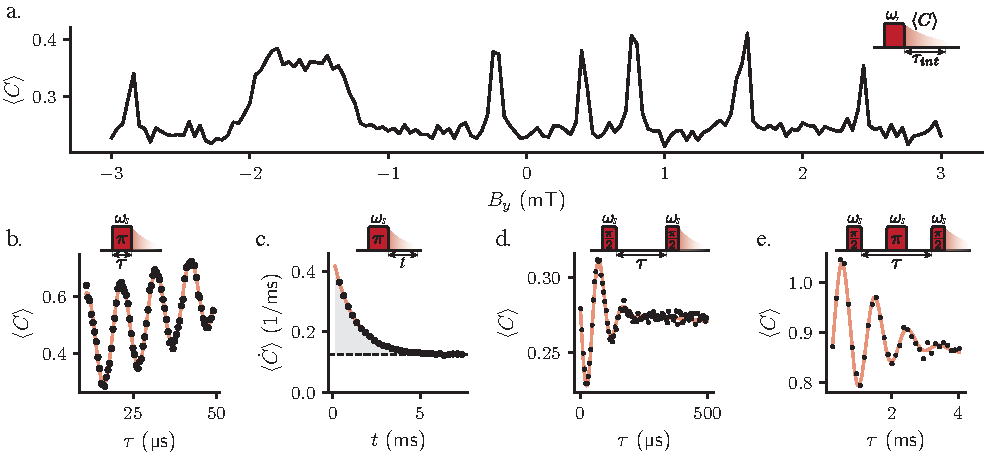
\includegraphics{chapter2/figures/electron_characterization.pdf}
    \caption[Low power spectroscopy and electron spin characterization]{Low power spectroscopy and electron spin characterization. Pulse sequences are shown as an inset in all subplots.
    \textbf{a.} Single spin spectroscopy. Ensemble average counts $\langle C \rangle$ as a function of $B_y$ measured with an integration time $\tau_\text{int}=10$~ms. The measurement data have been connected with a line for visual clarity. 
    \textbf{b.} Rabi sequence. $\langle C \rangle$ as a function of the duration of the driving pulse. The measurement was done with an integration time of 1~ms. The data is fit to a cosine oscillation with a linearly increasing background
    \textbf{c.} Single spin fluorescence. Count rate $\langle \dot C \rangle$ as a function of the time $t$ after a $\pi$ pulse. The data is fit to an exponential decay with a constant background. The integral of the data minus the background (gray area and dashed line respectively) gives a \textit{spin-to-click} efficiency $\eta_\text{spin}=0.39$. The fit yields $T_1=1.24$~ms from which we calculate the coupling $g_0/2\pi=4.5$~kHz.
    \textbf{d. \& e} Ramsey and Hahn echo sequence. $\langle C \rangle$ as a function of the interpulse delay $\tau$ between the two $\pi/2$-pulses. The exponentially decaying cosine fits yield $T_2^*=81$~\textmu s and $T_2=1.3$~ms respectively.
    }
    \labfig{electron_characterization}
\end{figure*}

We systematically characterize each \Er spin with the following measurements: 

\paragraph{Rabi oscillations} We measure $\langle C\rangle$ as a function of the duration of the driving microwave pulse (see \reffig{electron_characterization}b). On top of the Rabi oscillations, we note a linearly increasing background that we attribute the emission of unknown degrees of freedom~\sidecite{wang_addressing_2023}. The data is fit to a cosine oscillation with a linearly increasing background. The fit yields the Rabi frequency $\Omega$ for the specific microwave amplitude.

\paragraph{Fluorescence} We measure the count rate $\langle \dot C\rangle$ as a function of the time $t$ after the microwave pulse (see \reffig{electron_characterization}c). After the pulse, we wait a time $\tau_\text{w}=120$~\textmu s before measuring. The data is fit to a single exponential decay with a constant background. Given that the signal comes from a single emitter, the integral of the signal minus the background rate gives the \textit{spin-to-click} efficiency $\eta_\text{spin}$. During the experiments presented in this thesis, $\eta_\text{spin}\approx0.3-0.4$, a considerable improvement from previous demonstrations \sidecite{wang_singleelectron_2023}, thanks to the increased sensitivity of the SMPD used in this work \sidecite{pallegoix_enhancing_2025}. 

In addition, the fit yields the relaxation time of the spin $T_1$. For spins where the relaxation rate is completely dominated by the Purcell effect, we calculate the coupling to the resonator as 

\begin{equation}
    g_0 = \frac12 \sqrt{\frac{\kappa}{T_1}}
\end{equation}

In this work we measure $g_0/2\pi$ up to 9~kHz, a noticeable increase compared to ref.~\sidecite{wang_addressing_2023} where typical couplings ranged between 1--4~kHz. The enhanced coupling can be attributed to the narrower nanowire (see \refsec{sample_details}). This results in faster measurements, as the repetition time of the experiment is limited by the relaxation time of the spin $T_1$, which is proportional to $g_0^2$.

\paragraph{Ramsey and Hahn echo coherence}. We measure $\langle C\rangle$ after a Ramsey and a Hahn echo sequence as a function of the interpulse delay between the two $\pi/2$ pulses (see \reffig{electron_characterization}d \& e). The data are fit to an exponentially decaying cosine which yield the $T_2^*$ and $T_2$ respectively (see \refsec{effect_environment}). In the experiments we consistently observe $T_2^*\sim 100$~\textmu s and $T_2\sim1$~ms. Therefore, the coherence time is generally lifetime-limited. These extraordinary coherence times are consistent with the measurements performed by Marianne le Dantec in ensembles, where they achieve coherence times of $\sim20$~ms~\sidecite{ledantec_twentythreemillisecond_2021}. As discussed in \refsec{effect_environment}, this is possible thanks to the combination of low impurity concentration and the low nuclear magnetic moment density of \Ca.

\begin{figure*}
    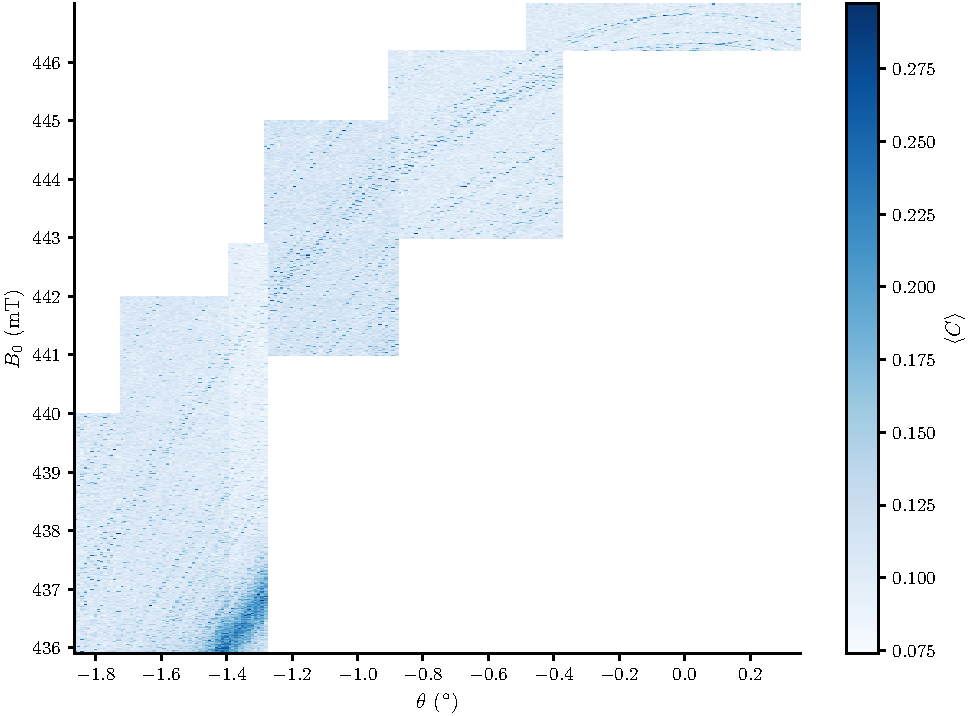
\includegraphics{chapter2/figures/2d_spectroscopy.pdf}
    \caption[2D single spin spectroscopy]{2D single spin spectroscopy. The map is created by stitching several individual measurements. Each measurement sweeps both the amplitude and the in-plane angle $\theta$ of the magnetic field. The SMPD is re-tuned to the resonator approximately every 0.5~mT. The total acquisition time was approximately 1 week}
    \labfig{2d_spectroscopy}
\end{figure*}

Finally, we measure a single-spin-resolved rotation pattern around $\theta = 0^\circ$. \reffig{2d_spectroscopy} presents a wide-range spectroscopic map concatenated from several measurement sets. We note that the span of the map is considerably larger than ones performed in ref.~\sidecite{wang_addressing_2023}. This increase is facilitated by the enhanced detection SNR granted by the larger coupling to the spin and improvements on the SMPD.

Individual \Er resonances are clearly resolved and each \Er spin has a slightly different gyromagnetic ratio. We associate this with inhomogeneous broadening discussed in \refsec{crystal_details}. The origin of the shifts likely originates  from local strain conditions, which arise due to differential thermal contractions from the metallic wire. Consequently, different spins are subject to different strain tensors depending on their spatial location with respect to the resonator wire. 

We note that the top of the parabolas of each spin do not lie at the same value of $\theta$. The strain distorts the $\gamma$-tensor, which likely loses its axial character. Nevertheless, there is a direction of minimal effective gyromagnetic tensor, but this direction can be slightly different for each \Er spin. In the following, we will call this direction the "local $c$-axis" of each spin.

%This observation is consistent with the correlation between enhanced coupling and increased inhomogeneous broadening reported in \sidecite{billaud_electron_2025}. This is explained by the proximity of the ions to the resonator surface. Spins located closer to the superconducting wire experience both stronger coupling and heightened local strain. This strain originates from the differential thermal contraction between the metallic resonator and the \Ca substrate when cooling the sample to 10~mK.

